\chapter{Články v časopisu Elektronka}
Ačkoliv se nejedná o podmínku hodnocení této práce, pro lepší pochopení této problematiky jsem začal psát články pro \href{https://www.spseol.cz/prace-zaku-a-studentu/casopis-elektronka}{školní časopis Elektronka}\cite{Elektronka} a obohacoval jimi tak svou rubriku \href{https://github.com/dlabaja/IT_doupe}{IT doupě}\cite{ITDoupe}. První vznikl v záři 2024 a mým úkolem je popsat od základů vytvořit web s tím, že každý měsíc do něj implementuju jinou technologii. Od primitivní HTML stránky se tak postupně dostávám k bundlingu, Reactu, Next.js, nebo lokalizacím.

\begin{figure}[!h]
    \centering
    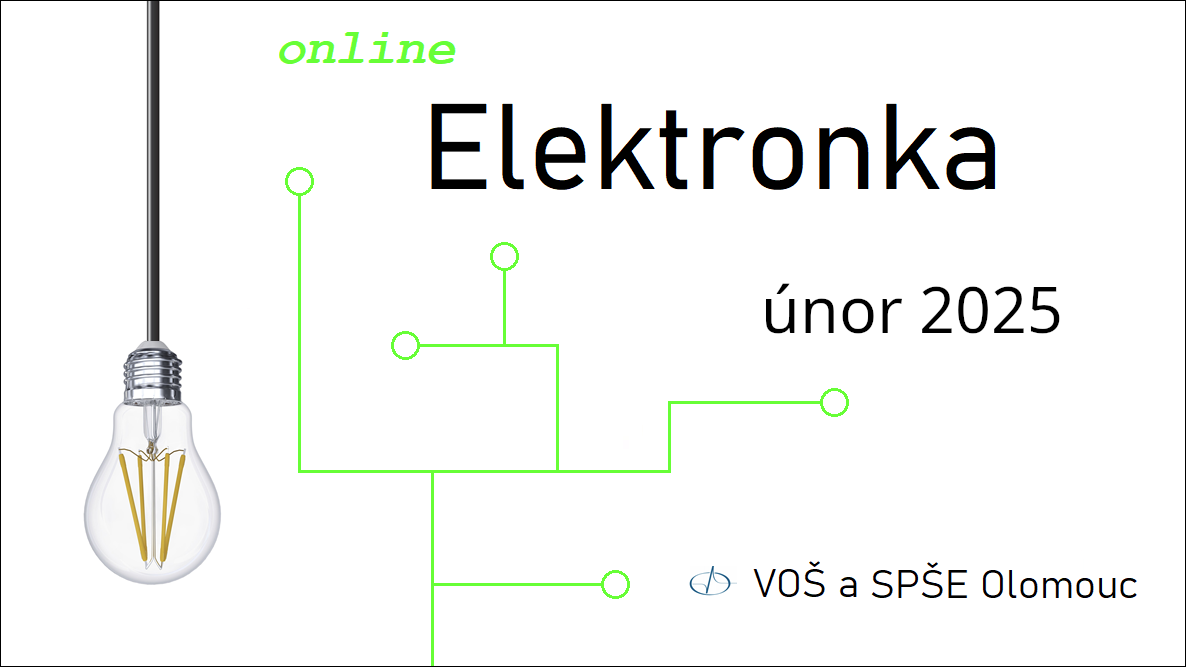
\includegraphics[width=1\linewidth]{obrazky/elektronka.png}
    \caption{Titulní obrázek časopisu Elektronka (únor 2025).\cite{Elektronka}}
\end{figure}
